% !TEX root =  ../main_manuscript.tex

\subsection{Study Population}
\label{subsec:study_population}
To develop our methodology we use the data of prostate cancer patients from the world's largest AS study called PRIAS \cite{bokhorst2016decade}. More than 100 medical centers from 17 countries worldwide contribute to the collection of data, utilizing a common study protocol and a web-based tool, both available at \url{www.prias-project.org}. We use data collected over a period of ten years, between December 2006 (beginning of PRIAS study) and December 2016. It consists of 5270 patients. The primary event of interest in this work is cancer progression detected upon a positive biopsy. It is observed in 866 patients, although the time of cancer progression is interval censored because biopsies are scheduled periodically. Biopsies are scheduled as per the PRIAS protocol (see \hyperref[sec:introduction]{Introduction}). There are three types of competing events, namely death of 63 patients, of which 61 died from reasons unrelated to prostate cancer; removal of 464 patients from AS on the basis of their observed DRE and PSA measurements; and loss to follow-up of 685 patients because of patient anxiety or unknown reasons. In this work, we assume these three types of events to be censoring (see Appendix~A.5 for details). However, our model allows removal of patients to depend on observed longitudinal data and baseline covariates of the patient. Under the aforementioned assumption of censoring, Figure~\ref{fig:npmle_plot} shows the cumulative risk of cancer progression over the study follow-up period.

\begin{figure}[!htb]
\captionsetup{justification=justified}
\centerline{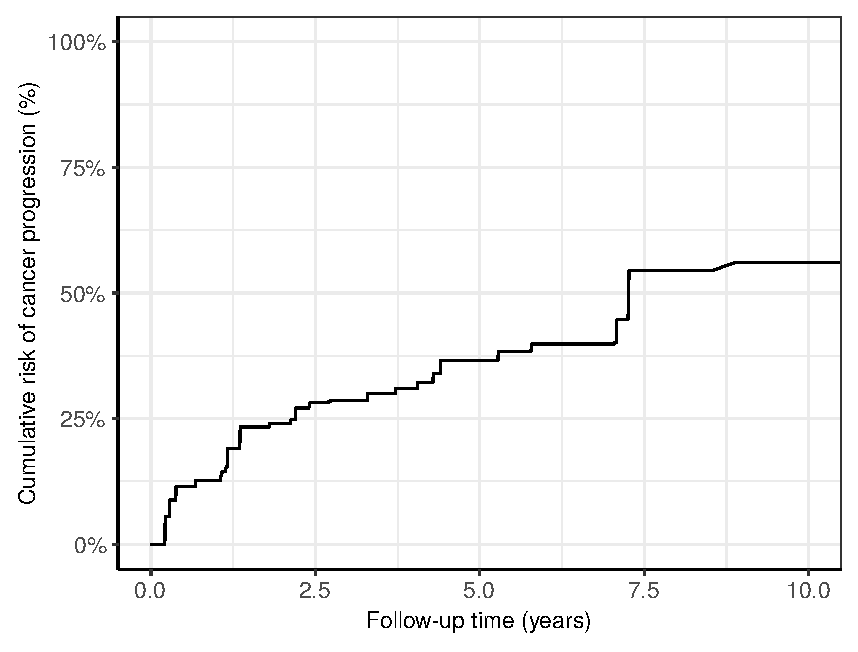
\includegraphics[width=\columnwidth]{images/npmle_plot.eps}}
\caption{\textbf{Estimated cumulative risk of cancer progression in AS} for patients in the Prostate Cancer Research International Active Surveillance (PRIAS) dataset. Nearly 50\% patients (\textit{slow progressing}) do not progress in the ten year follow-up period. Cumulative risk is estimated using nonparametric maximum likelihood estimation \citep{turnbull1976empirical}, to account for interval censored cancer progression times observed in PRIAS program. Censoring includes death, removal from AS on the basis of observed longitudinal data, and patient dropout.}
\label{fig:npmle_plot}
\end{figure}

For all patients, PSA measurements (ng/mL) are scheduled every 3 months for the first 2 years and every 6 months thereafter. The DRE measurements (ordinal scale) are scheduled every 6 months. We use the DRE measurements after converting them to a binary scale, namely $\mbox{DRE} > \mbox{T1c}$ and $\mbox{DRE} = \mbox{T1c}$. A DRE measurement equal to T1c\cite{schroder1992tnm} indicates a clinically inapparent tumor which is not palpable or visible by imaging. Tumors with $\mbox{DRE} > \mbox{T1c}$ are palpable. On average 5 DRE and 9 PSA measurements have been recorded per patient. 




